We discuss the design of the codes for creating extra accesses to memory in this section. First we discuss the code designs explored during Phase I. Second, we discuss specific execution strategies to efficiently implement the designs.\\
In this part, we attempt to design efficient codes based on the memory traces shared by Huawei. The goal of this design was to simulate the efficiency of coding and compare the results to the baseline implementation of not coding. During this design phase, we explored various code functions that could be used to create the codes on the stored data. We decide upon using the XOR function to store the data in the parity banks because of it�s low complexity overhead and for preserving the linearity of codes. Linear codes offer the widest range of functionality because any order of the codes may be used to either encode or decode. This lack of dependency allows our design to use the parity banks in the most flexible way possible. We also explore the potential benefits of using different weights to the memory elements for the XOR function. For examples, the memory elements $a_0$ and $b_0$ could be stored as $\alpha a_0 + \beta b_0$ for any integer value of $\alpha$ and $\beta$. The least complex design for the decoder would be for taking $\alpha$ = 1 and $\beta$ = 1 . Another design consideration explored is the compression factor to generate the codes. The codes can be generated by using xor on 2 or more memory elements. For example, suppose there are four banks A, B , C and D. Each of the banks hold $a_0$ to $a_n$, $b_0$ to $b_n$ , $c_0$ to $c_n$ and $d_0$ to $d_n$ elements respectively. The possible codes for these memories could be:
\begin{equation}
a_i + b_i, b_i + c_i, c_i + d_i \text{ and } c_i + a_i  \text{ for i = 0 to n }
\end{equation}
This scheme uses the combination of 2 memory elements to generate the codes. Although this requires 100$\%$ extra memory overhead, it enables 100$\%$ extra memory accesses per cycle, i.e., 4 extra accesses in this case.
Another design could be to compress the codes by combining all 4 memory elements to generate the codes:
\begin{equation}
a_i + b_i + c_i + d_i \text{ for i = 0 to n }
\end{equation}
This design gives one extra access per cycle at the cost of 25$\%$ memory overhead. However, the decoder here needs to know 3 elements to be able to decode the 4th element. So although we are able to compress more data into a single memory location, it comes with the cost of additional memory logic. 
The scheme described above "codes" the memory banks using elements from different banks. We call this type of coding as Interbank Coding. We also explore the orthogonal way of coding, i.e. intra-bank coding where we use the memory elements from the same bank to generate codes.
\\
Next, we explore the code design for the following objectives:
\begin{itemize}
\item Read access : 4 per bank in one cycle
\item Write access : 2 per bank in one cycle
\item Shared Memory size 8 kB - 256 kB
\item Number of Banks : 8
\item Memory overhead : 15$ \% $
\item Parity banks : 5 or 6 shallow banks for code storage
\end{itemize}
Using the above parameters, we design coding scheme to efficiently store the codes and achieve the objective. We use the concept of batch codes to code specific areas within each of the banks. This allows us to serve multiple accesses to the coded region using the parity banks. With this scheme, we guarantee that any 4 requests to the coded region can be served at any given time. As shown in figure~\ref{fig:design2} , 8 banks are divided into two regions. Each region consists of 4 banks. Each region has 6 parallel shallow  banks to store the parity. The colored regions shown in the banks 1-8 are the coded region. These regions are assumed to be of a fraction of the memory. \\ 
\textit{Best case scenario}: We design this code to achieve maximum performance when sequential accesses to the coded regions are issued. During the best case access, we can achieve up to 10 parallel accesses in one cycle. Consider the scenario if we receive accesses to $a_1,b_1,c_1,d_1,a_2,b_2,c_2,d_2,a_3,b_3,c_3,d_3$. Here, we can serve $a_1,b_1,c_1,d_1$ using a1 with the parity banks $a_1+b_1,b_1+c_1,c_1+d_1$ and serve $a_2$,$b_2$,$c_2$,$d_2$ using $b_2$ with the parity banks $b_2$+$c_2$,$b_2$+$d_2$,$a_2$+$c_2$. Lastly, we can serve $c_3$ and $d_3$ using bank 3 and bank 4. \\
\begin{figure}[ht!]
\centering
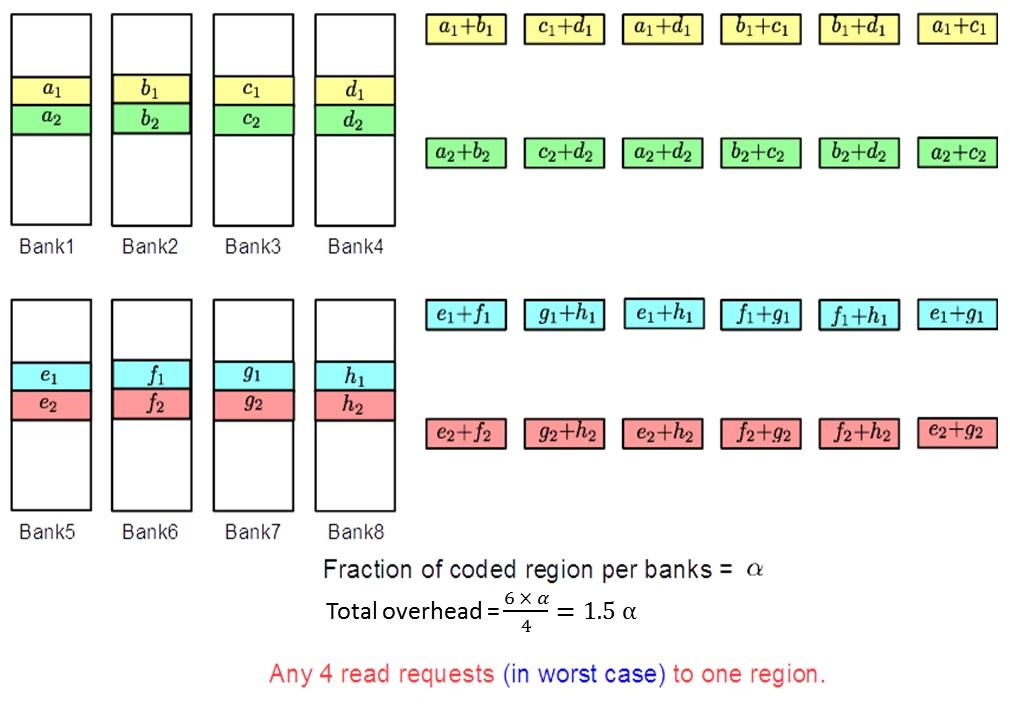
\includegraphics[width=90mm,natwidth=610,natheight=642]{simple_design1.jpg}
\caption{ }
\label{fig:design1}
\end{figure} 
\begin{figure}[ht!]
\centering
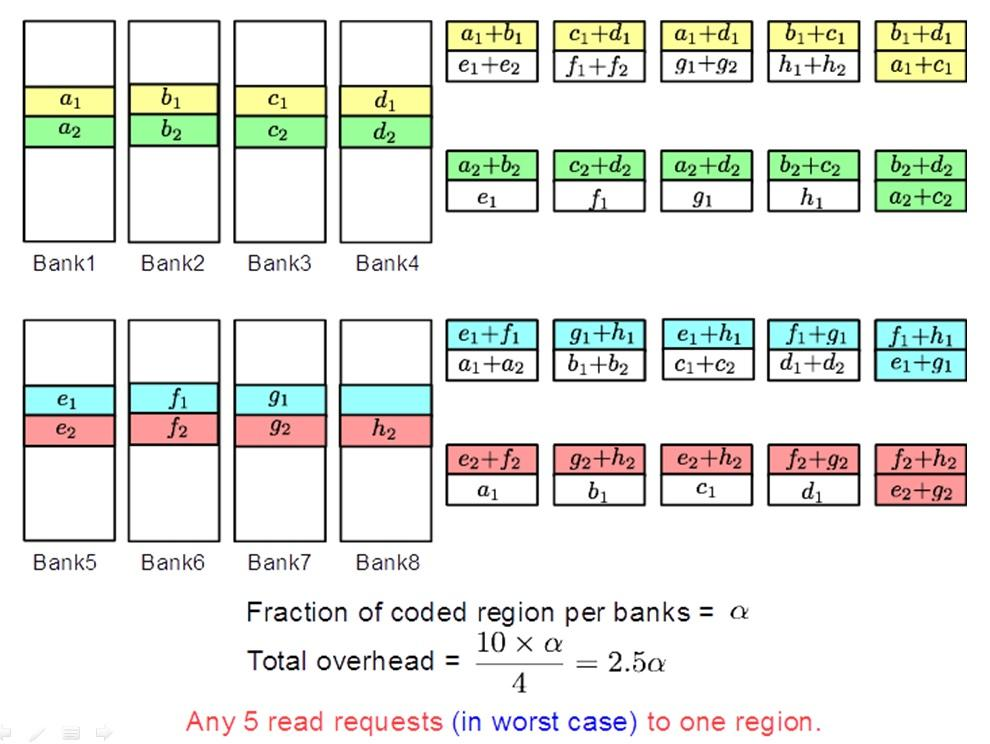
\includegraphics[width=90mm,natwidth=610,natheight=642]{design2.jpg}
\caption{ }
\label{fig:design2}
\end{figure}
\begin{figure}[ht!]
\centering
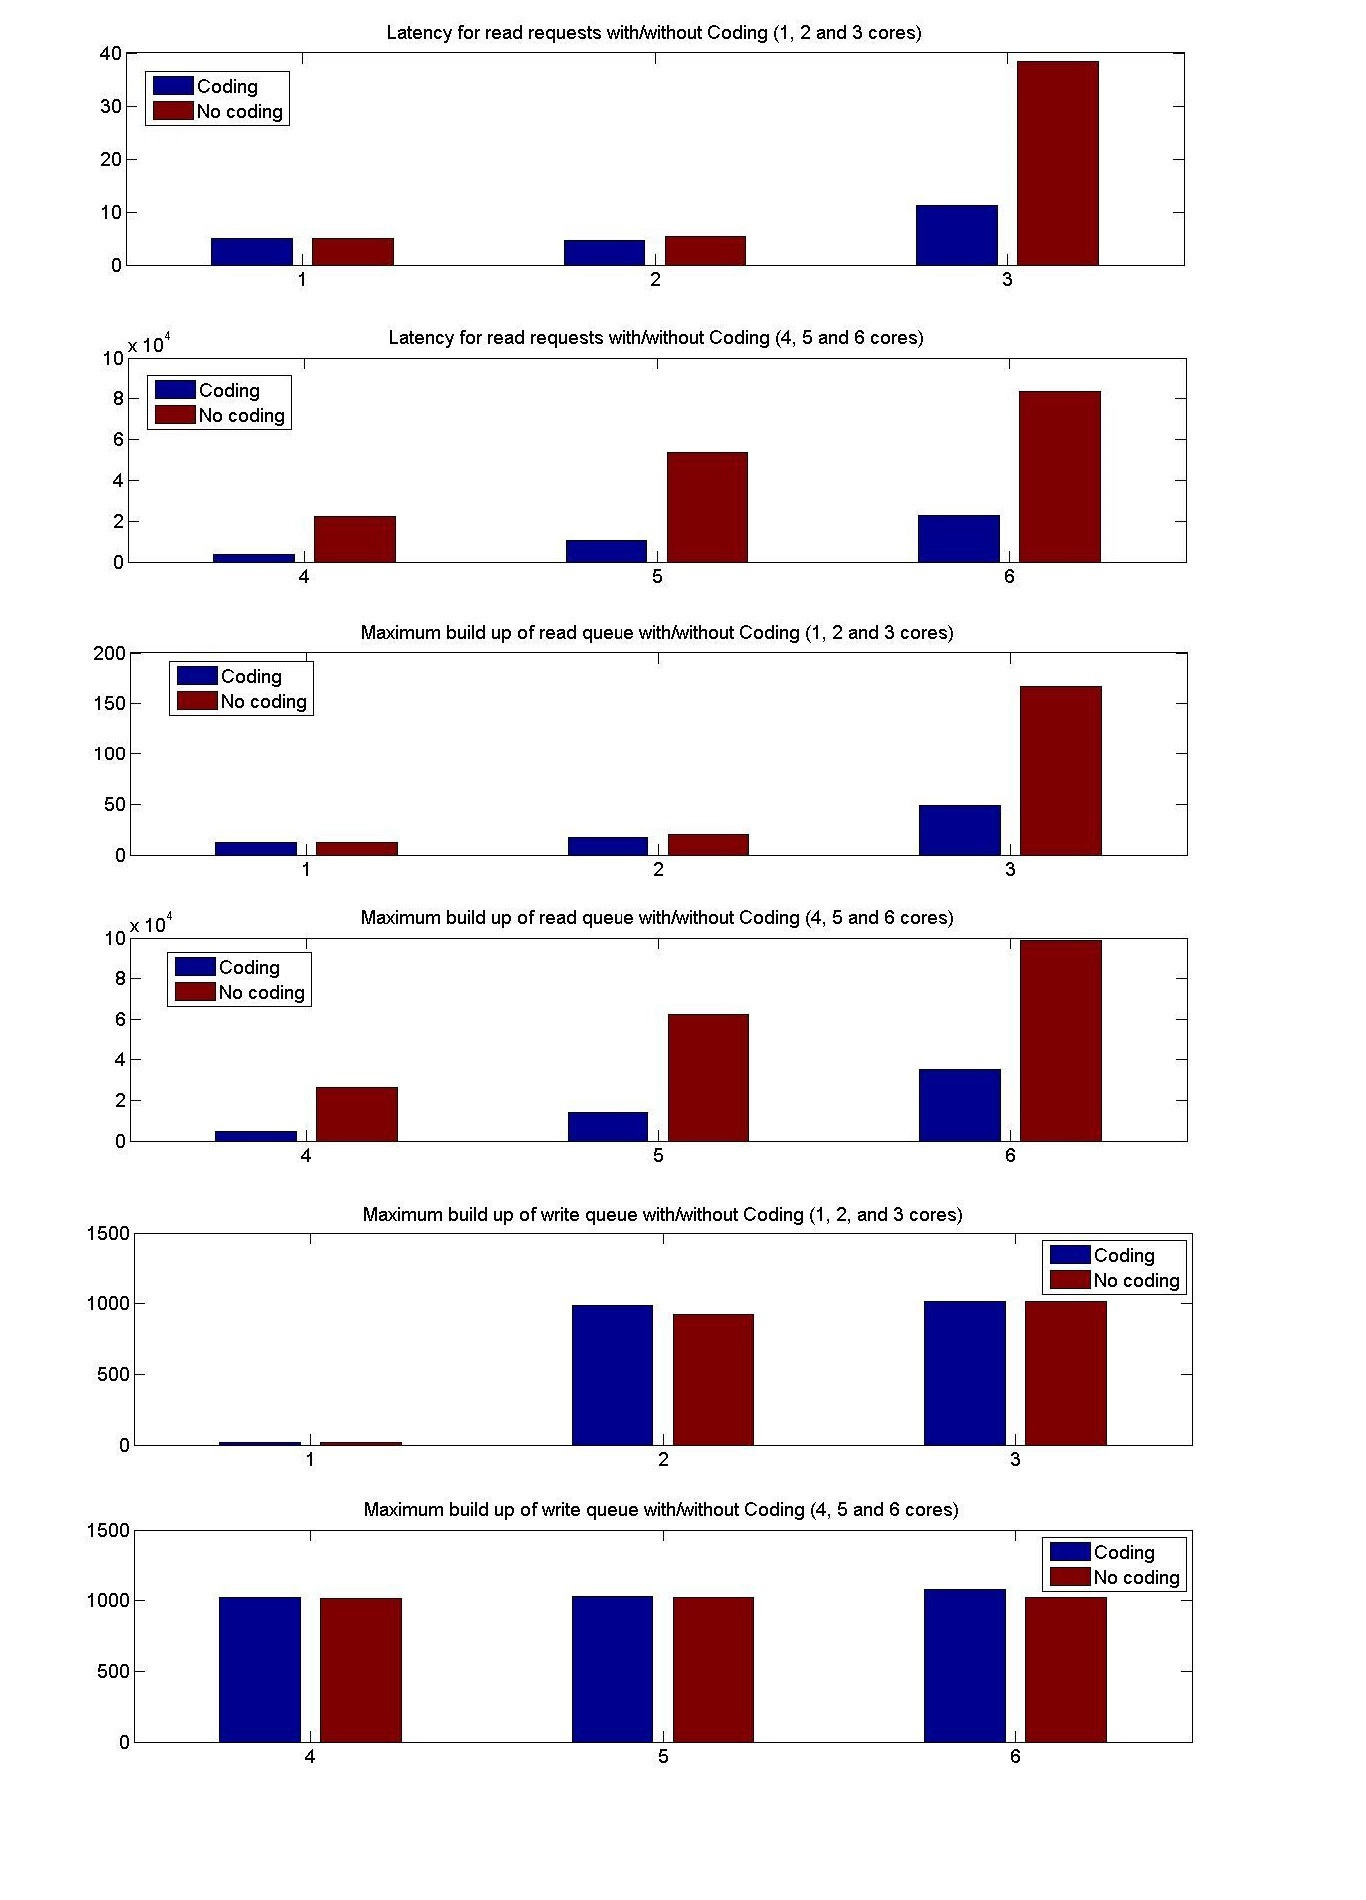
\includegraphics[width=150mm,natwidth=610,natheight=642]{result_design1.jpg}
\caption{ }
\label{fig:result_design1}
\end{figure}
\\ 
\textit{Worst Case analysis}: The code scheme falls off to 4 access in a cycle when there are non-sequential and non-consecutive access to the memory banks. For example when the access pattern is to a1, b8,c9,d15. Since we do not code this combination, it does not get benefit of extra access. However in this case, we can use the prefetching mechanism to look ahead in the queue and prefetch codes from parity banks for the subsequent access. 
In Figure~\ref{fig:result_design1} , we explore the worst case scenario when the accesses are random. The results show that the queue build up for reads and writes does fall back to no-coding scenario. This asserts that the worst case scenario for a coding scheme performs similar to no-coding scheme .
  
In the second scheme, we augment the code storage by cross storing the codes from region 1 to region 2 and vice versa. We do this in addition to coding the consecutive memory addresses in a bank. This provides two benefits, first it increases the overall redundancy, and second it allows us to use the parity banks of the other region in case the first region�s parity banks are in use. Figure~\ref{fig:design2} shows the storage pattern of the codes in the bank.  The overall overhead in this system is 2.5a.
\begin{figure}[ht!]
\centering
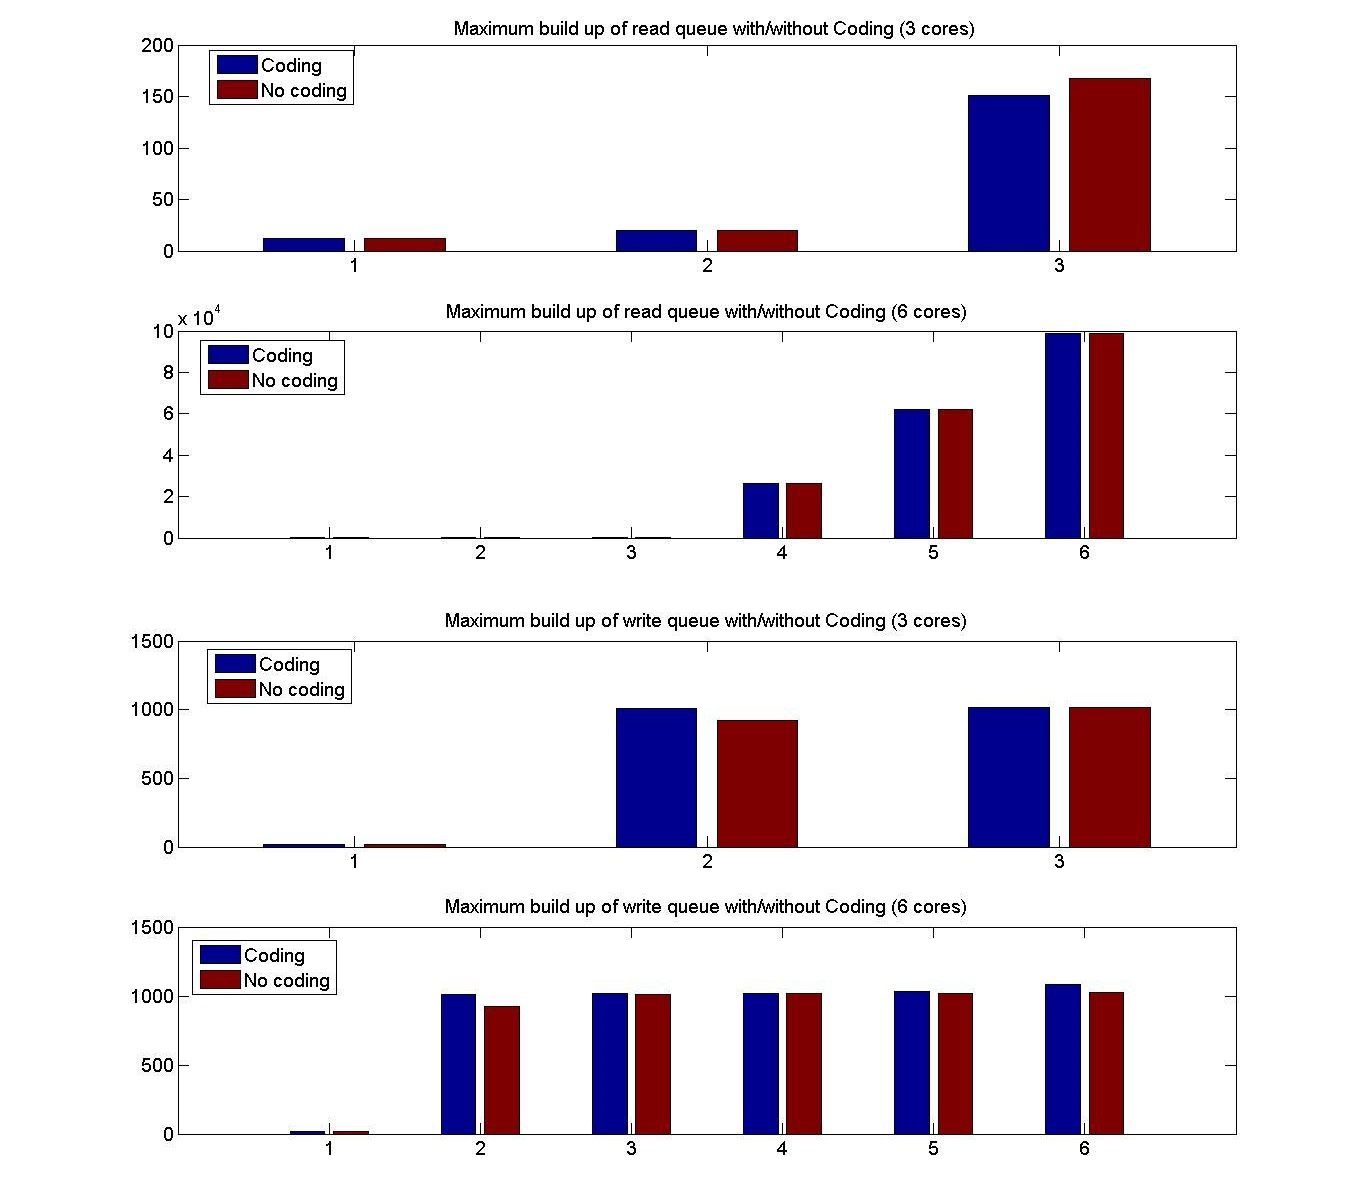
\includegraphics[width=150mm,natwidth=610,natheight=642]{result_design2.jpg}
\caption{ Comparison of Design II with No coding case }
\label{fig:result_design2}
\end{figure}
\textit{Best case analysis}: We design this code to achieve maximum performance when sequential accesses to the coded regions are issued. During the best case access, we can achieve up to 9 parallel accesses in one cycle. Consider the scenario if we receive accesses to $a_1,b_1,c_1,d_1,a_2,b_2,c_2,d_2,a_3,b_3,c_3$. Here, we can serve $a_1, b_1, c_1, d_1$ using $a_1$ with the parity banks $a_1+b_1,b_1+c_1,c_1+d_1$ and serve $a_2,b_2,d_2$ using $b_2$ with the parity banks $a_2+d_2$ and $b_2+d_2$. Lastly, we can serve $c_2$ and $d_3$ using bank 3 and bank 4. 

\textit{Worst Case analysis}: The code scheme can do 5 accesses in a cycle for the coded region in worst case. These are non-sequential and non-consecutive accesses to the memory banks. For example, when the access pattern is $a_1,a_6,a_9,a_{15},a_{20}$, we can perform these 5 reads with the help of coded banks. We can use the prefetching mechanism discussed later to look ahead in the queue and pre-fetch codes from parity banks for the subsequent access. 

